\documentclass[a4paper,12pt]{article}
%\usepackage{fullpage}
%\usepackage{pdfpages}

\usepackage{geometry}
 \geometry{
 a4paper,
 total={170mm,257mm},
 left=20mm,
 top=20mm,
 }

\usepackage{color}
\usepackage{amsmath,graphicx,makeidx}
\usepackage{lscape}
\usepackage{fancyhdr}
\addtolength{\headheight}{1.5cm} % make more space for the header
\pagestyle{fancyplain} % use fancy for all pages except chapter start
\lhead{
\includegraphics[height=1.7cm]{FOSSEE-logo}} % left logo
\rhead{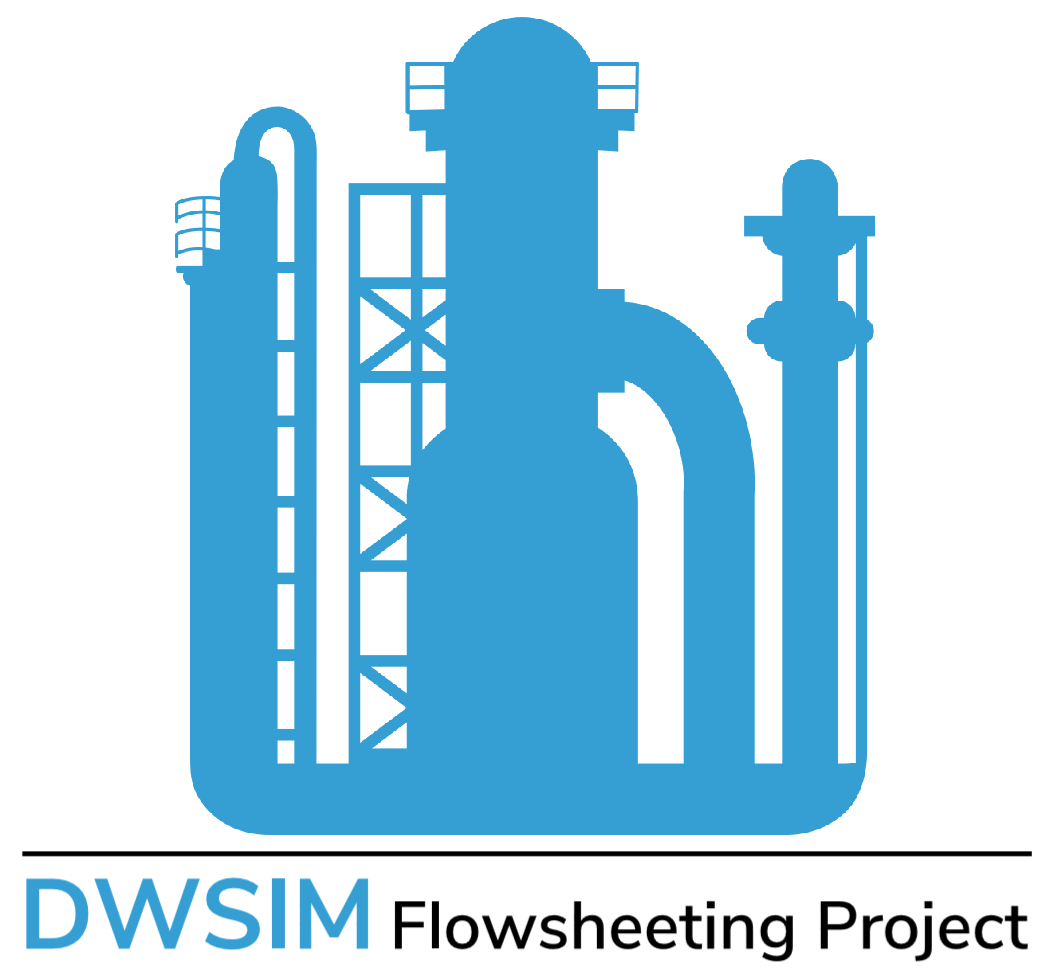
\includegraphics[height=3.5cm]{DWSIM-flowsheeting-project-logo}} % right logo
\renewcommand{\headrulewidth}{0pt} % remove rule below header

\title{Pressure Swing Azeotropic Distillation of Methanol-Acetone}
\author{Priyam Nayak \\ Indian Institute of Technology Bombay}
\date{}

\begin{document}

\maketitle

\noindent \textbf{Background \& Description:}
\newline Pressure swing distillation is one of the most common methods for separating a binary homogeneous azeotrope. This method is preferred when the composition of the azeotrope changes with pressure. 


In this process, equimolar amount of methanol - acetone mixture enters a low pressure column (LPC) at 300 K temperature and 1 bar pressure. The column consists of 52 stages including the condenser and reboiler. Feed enters at the 37$^{th}$ stage. The low pressure column operated at 1 bar. The column is operated at reflux ratio of 2.36. The distillate from the first column gives an azeotrope with 75\% acetone (mol basis). The temperature of the top product is around 314 K. The bottoms from the column gives methanol with 99.5\% purity. The top product from the LPC is pumped into a high pressure column (HPC) operating at 10 bar. The HPC consists of 62 stages with the pumped feed entering at 41$^{st}$ stage. The column is operated at reflux ratio of 3.11. The bottoms from the HPC gives 99.4\% acetone. The distillate from the HPC comprising 60\% methanol is recycled to the LPC at the 41st stage.


\vspace{25mm}
\centerline{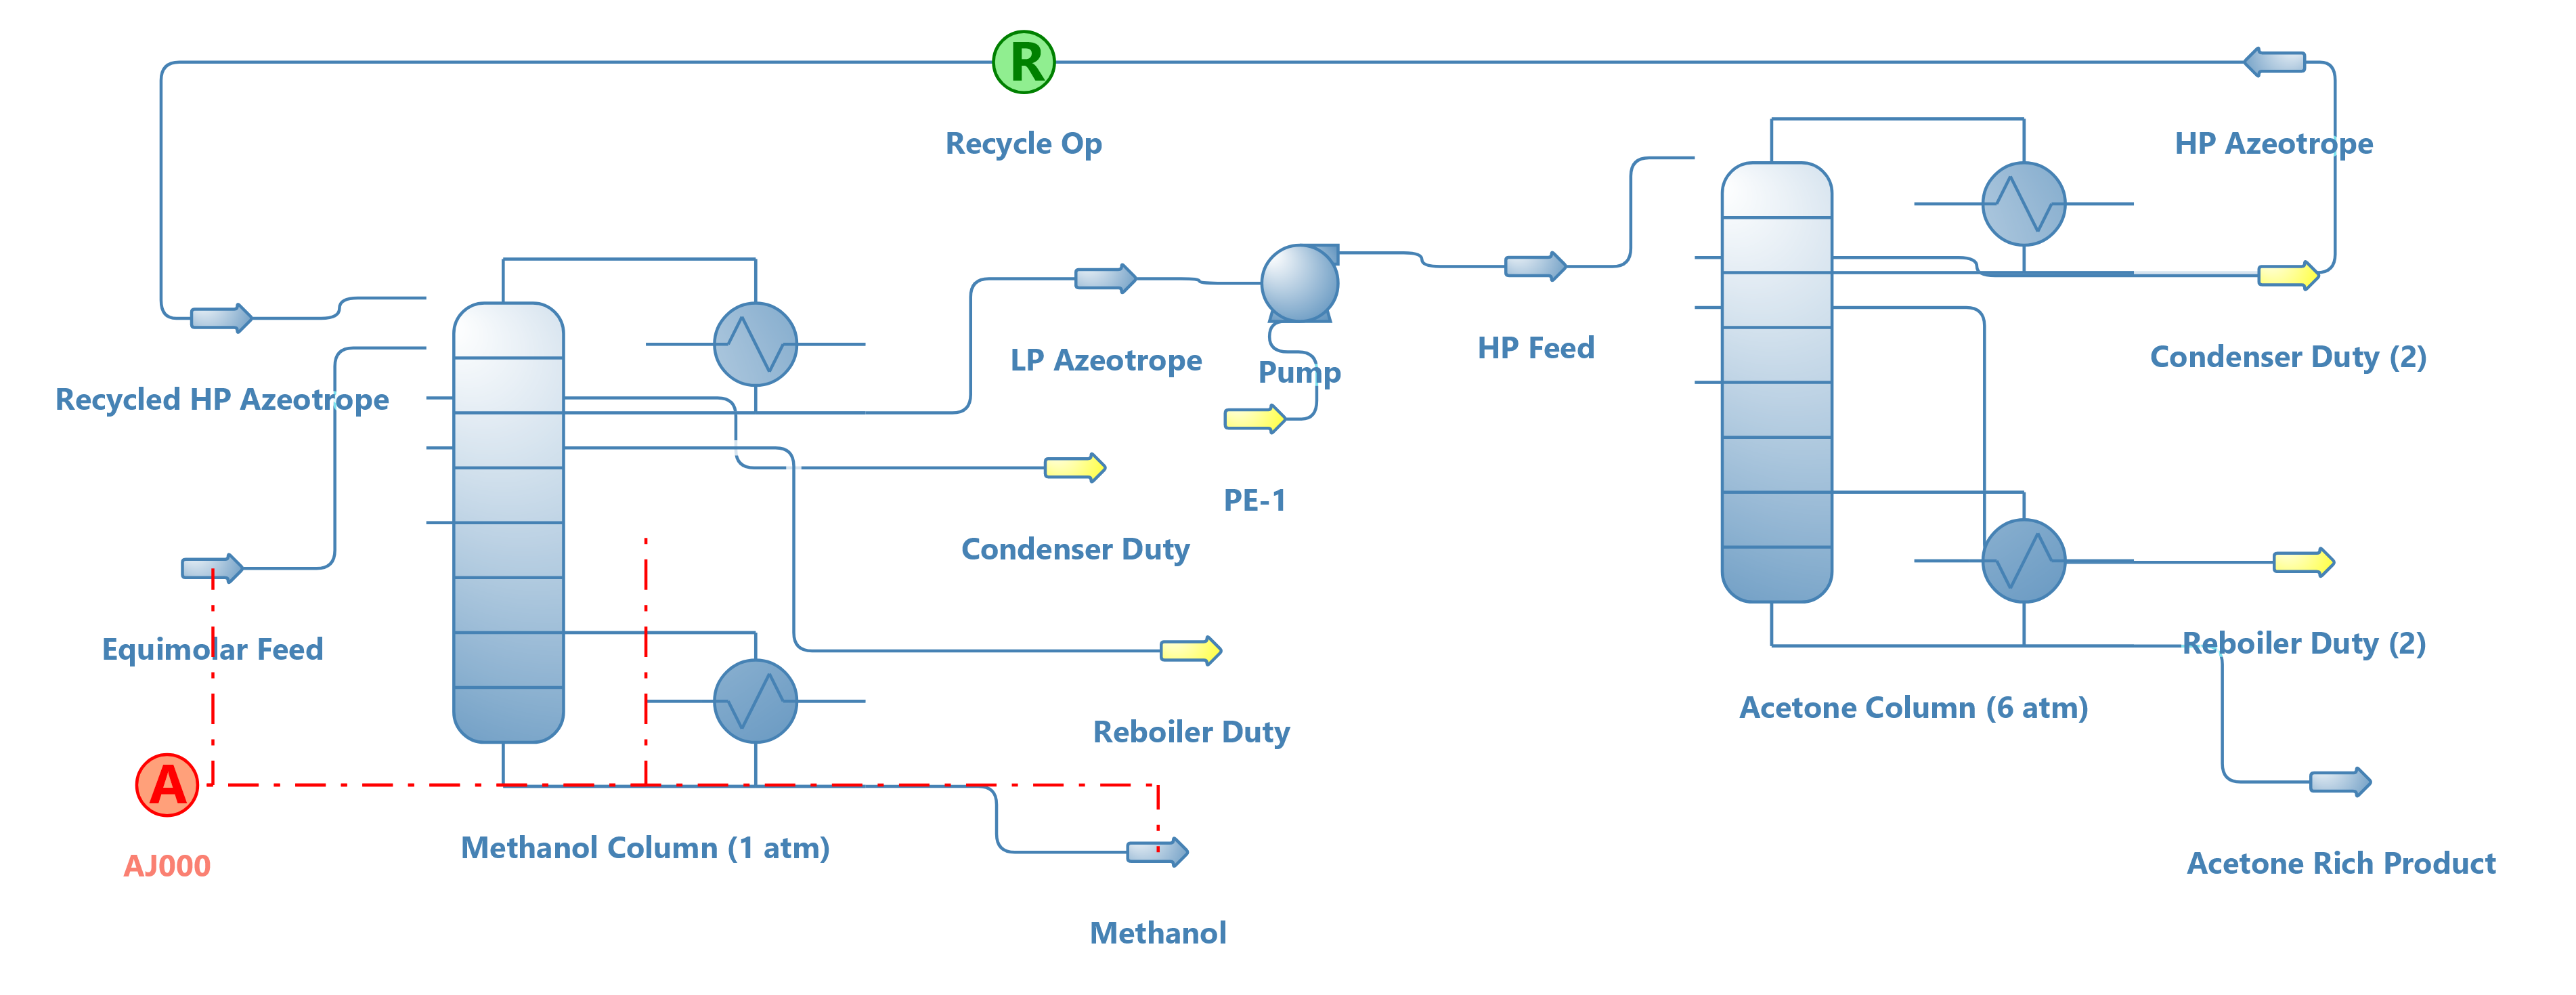
\includegraphics[width=0.85\linewidth]{PSD-Methanol-Acetone.png}}

\newpage
\noindent \textbf{Results:}
\begin{table}[ht]
\centering
\resizebox{\textwidth}{!}{%
\begin{tabular}{|l|l|l|l|l|l|l|l|l|}
\hline
Object                                & Recycled HP & Methanol & LP Azeotrope & HP Feed  & HP Azeotrope & Equimolar & Acetone &       \\ 
                                &  Azeotrope & Methanol & LP Azeotrope & HP Feed  & HP Azeotrope & Feed & Rich Product &       \\ \hline
Temperature                           & 394.949               & 337.9007 & 329.8019     & 330.0324 & 394.949      & 300            & 394.949              & K     \\ \hline
Pressure                              & 607950                & 101325   & 101325       & 607950.1 & 607950       & 101325         & 607950               & Pa    \\ \hline
Mass Flow                             & 0.11068               & 0.01602  & 0.13975      & 0.13975  & 0.11068      & 0.045          & 0.02904              & kg/s  \\ \hline
Molar Flow                            & 1.90569               & 0.5      & 2.40619      & 2.40619  & 1.90569      & 0.9986         & 0.5                  & mol/s \\ \hline
Molar Fraction &                      &         &             &         &             &             &                     &       \\
(Mixture)  /  Methanol & 0                     & 1        & 0            & 0        & 0            & 0.5            & 0                    &       \\ \hline
Molar Fraction &                      &         &             &         &             &             &                     &       \\
(Mixture)  /  Acetone  & 1                     & 0        & 1            & 1        & 1            & 0.5            & 1                    &       \\ \hline
\end{tabular}%
}
\caption{Streamwise Results for Pressure Swing Distillation of Methanol-Acetone}
\end{table}

\end{document}


